\section{Behaviour of Model under Parameter Changes}
\label{sec:yunus.param.effects}

In this section, we examine the effects of the parameters on the function of the original model.
Starting with the combined effects of the parameters along areas of the same period.
And then also the individual effects of either parameter.

\subsection{Combined Effects of Parameters}
\label{sec:yunus.param.effects.combined}

To replicate the dynamics seen in the model, it is helpful to know, how the model changes along the areas of the same period.
\Cref{fig:yunus.function.evolution.12} shows, how the model function changes along the area of period 12.
In the figure, there are three functions in three different colors.
The first function is blue and it is the model with parameters $E_0 = 15.9, \chi_0 = 0.11$, it is marked as point $A_12$ in \Cref{fig:yunus.function.evolution.map}.
The second function is purple and it is the model at the point $E_0 = 17.07, \chi_0 = 0.182$, marked as point $B_{12}$.
The last function is red and it is the model with parameters $E_0 = 18.5, \chi_0 = 0.27$, marked as point $C_{12}$.

\begin{figure}
    \centering
    \begin{subfigure}{0.4\textwidth}
        \includegraphics[width=\textwidth]{99_Yunus/2D_Period_Zoomed_Effects/result.png}
        \caption{Measured Points}
        \label{fig:yunus.function.evolution.map}
    \end{subfigure}
    \begin{subfigure}{0.4\textwidth}
        \includegraphics[width=\textwidth]{99_Yunus/ParameterEffects/E0_hi_P12/illustration.png}
        \caption{Evolution for Period 12}
        \label{fig:yunus.function.evolution.12}
    \end{subfigure}
    \begin{subfigure}{0.4\textwidth}
        \includegraphics[width=\textwidth]{99_Yunus/ParameterEffects/E0_hi_P10/illustration.png}
        \caption{Evolution for Period 10}
        \label{fig:yunus.function.evolution.10}
    \end{subfigure}
    \begin{subfigure}{0.4\textwidth}
        \includegraphics[width=\textwidth]{99_Yunus/ParameterEffects/E0_hi_P08/illustration.png}
        \caption{Evolution for Period 8}
        \label{fig:yunus.function.evolution.08}
    \end{subfigure}
    \caption{Effects of the Parameters on the Original Funtion}
\end{figure}

The most notable changes are
\begin{enumerate*}
    \item Branches $\A$ and $\C$ move upwards while the left part moves upwards more
    \item The left part of branches $\B$ and $\D$ move downwards 
    \item The local minima of these branches move to the left and downwards.
\end{enumerate*}
One smaller change is that the border between branches $\B$ and $\C$ moves left.
Note that the same change happens to the border between the branches $\D$ and $\A$.

The same effects can be observed for the areas of period 8 and 10.
The effects are visualized in \Cref{fig:yunus.function.evolution.10,fig:yunus.function.evolution.08}.
The points used for measurement are visualized in \Cref{fig:yunus.function.evolution.map}.
For the period 10, points $A_{10}, B_{10},$ and $C_{10}$ are used and for period 8, points $B_8$ and $C_8$.

\subsection{Individual Effects of Parameters}
\label{sec:yunus.param.effects.individual}

The effects of the parameters described above, always include a change in both parameters $E_0$ and $\chi_0$.
To reproduce the bifurcation structures, it is important to know which effects on the function each parameter has individually.

\begin{figure}
    \centering
    \includegraphics[width=0.4\textwidth]{99_Yunus/2D_Period_Zoomed_EffectsSingle/result.png}
    \label{fig:yunus.function.evolution.single.map}
    \caption{Parameter Ranges Scanned for Individual Effects of Parameters}
\end{figure}

For the parameter $E_0$, we fixed $\chi_0 = 0.2$ and varied $E_0$ in the parameter range $[15, 19]$, it is marked as the green arrow in \Cref{fig:yunus.function.evolution.single.map}.
Like before, we took the function at three points and put them in one figure with color codes.
\Cref{fig:yunus.function.evolution.e0} shows this.
The blue function is the function of the original model at the start of the parameter range, $E_0 = 15$ and $\chi_0 = 0.2$.
The purple function is in the middle at $E_0 = 17$ and $\chi_0$ stays the same.
And the red function is at the end at $E_0 = 19$.
From the figure we can see three effects, the parameter has on the function of the original model in this parameter range.
The observed changes are
\begin{enumerate*}
    \item The left part of branches $\B$ and $\D$ move downwards
    \item The local minima of these branches move to the left and downwards
    \item The border between branches $\A$ and $\B$ moves right (also border between branches $\C$ and $\D$)
    \item The Right side of branches $\A$ and $C$ move up (This is a direct effect of the border between branches $\A$ and $\B$ moving right).
\end{enumerate*}

For the parameter $\chi_0$, we fixed $E_0 = 17$ and varied $\chi_0$ in the parameter range $[0.125, 0.3]$.
This parameter range is marked orange in \Cref{fig:yunus.function.evolution.single.map}.
The function is displayed at three points of the parameter range in \Cref{fig:yunus.function.evolution.hi}.
As before, the blue function is the function of the original model at the start of the parameter range, $E_0 = 17$ and $\chi_0 = 0.125$.
The purple function is at $\chi_0 = 0.2125$, and the red one is at $\chi_0 = 0.3$.
The observed changes are
\begin{enumerate*}
    \item The branches $\A$ and $\C$ move upwards
    \item The border between $\A$ and $\B$ moves left (also the border between branches $\C$ and $\D$).
\end{enumerate*}
Two more changes are smaller in comparison
\begin{enumerate*}
    \item The right part of branches $\B$ and $\D$ move upwards (including the minima)
    \item The border between branches $\B$ and $\C$ moves left (also the border between branches $\D$ and $\A$).
\end{enumerate*}

\begin{figure}
    \centering
    \begin{subfigure}{0.4\textwidth}
        \includegraphics[width=\textwidth]{99_Yunus/ParameterEffects/E0/illustration.png}
        \caption{Evolution for Parameter $E_0$}
        \label{fig:yunus.function.evolution.e0}
    \end{subfigure}
    \begin{subfigure}{0.4\textwidth}
        \includegraphics[width=\textwidth]{99_Yunus/ParameterEffects/hi/illustration.png}
        \caption{Evolution for Parameter $\chi_0$}
        \label{fig:yunus.function.evolution.hi}
    \end{subfigure}
    \caption{Effects of the Individual Parameters on the Original Funtion}
\end{figure}

\subsection{Decomposition of Combined Effects}
\label{sec:yunus.param.effects.decomposition}

Now we can take a closer look at the combined effects of the parameters along areas of the same period and trace them back to the isolated effects of both parameters.
For this, we introduce a notation for the effects.
The effect of moving the left side of a branch up is denoted $\AL$, for the right side $\AR$, and for the whole branch $\AW$
The subscript indicates, which branch the change effects, and the superscript indicates, whether the branch moves upwards $+$ or downwards $-$.
The effect of moving a local minimum is denoted as $\AMi$.
The meaning of the subscript stays the same as above, but the superscript also can include $L$ for left and $R$ for right.
Finally, the effect of moving borders is denoted as $\AB$.
The subscript now includes the two branches, to which the border belongs, and the superscript now has only $L$ or $R$.
For brevity, we do not write redundant branch names, so changes happening to branch $\A$ are also happening to branch $\C$.
For borders, changes to the border between branches $\A$ and $\B$ are also happening to the border between branches $\C$ and $\D$.

\Cref{tab:yunus.parameter.effects} lists all observed effects along the areas of the same period and their decomposition into effects of the single parameters.
The first part of the table includes all major changes observed in \Cref{sec:yunus.param.effects.combined}, while the second part focuses on the minor change.
The second part also includes the changes observed in \Cref{sec:yunus.param.effects.individual} that cancel out.
From this table we can see, that $E_0$ causes the feects on the branches $\B$ and $\D$, while $\chi_0$ causes the changes to the branches $\A$ and $\C$, as well as the minor movement of the borders between branches $\B$ and $\C$.
Note again, that the change to the border of branches $\B$ and $\C$ also applies for the border between branches $\D$ and $\A$.

\begin{table}
    \centering
    \begin{tabular}{|c|c|c|l|} \hline
        Combined & $E_0$ & $\chi_0$ & Comment \\ \hline \hline
        $\AL_{\B}^{-}$ & $\AL_{\B}^{-}$ & 0 & Only $E_0$ causes this \\ \hline
        $\AMi_{\B}^{L-}$ & $\AMi_{\B}^{L-}$ & $-\AMi_{\B}^{+}$ &
            $E_0$ and $\chi_0$ have opposing effects, the effect of $E_0$ is stronger \\ \hline
        $\AW_{\A}^{+}$ & 0 & $\AW_{\A}^{+}$ & Only $\chi_0$ causes this \\ \hline \hline
        $\AB_{\B\C}^{L}$ & 0 & $\AB_{\B\C}^{L}$ & Only $\chi_0$ causes this \\ \hline
        0 & $\AB_{\A\B}^{R}$ & $-\AB_{\A\B}^{L}$ &
            $E_0$ and $\chi_0$ have opposing effects, they cancel out \\ \hline
    \end{tabular}
    \caption{Decomposition of Combined Effects of Parameters}
    \label{tab:yunus.parameter.effects}
\end{table}
